\section{Semantic Search}
\begin{figure}[tbh]
	\centering
		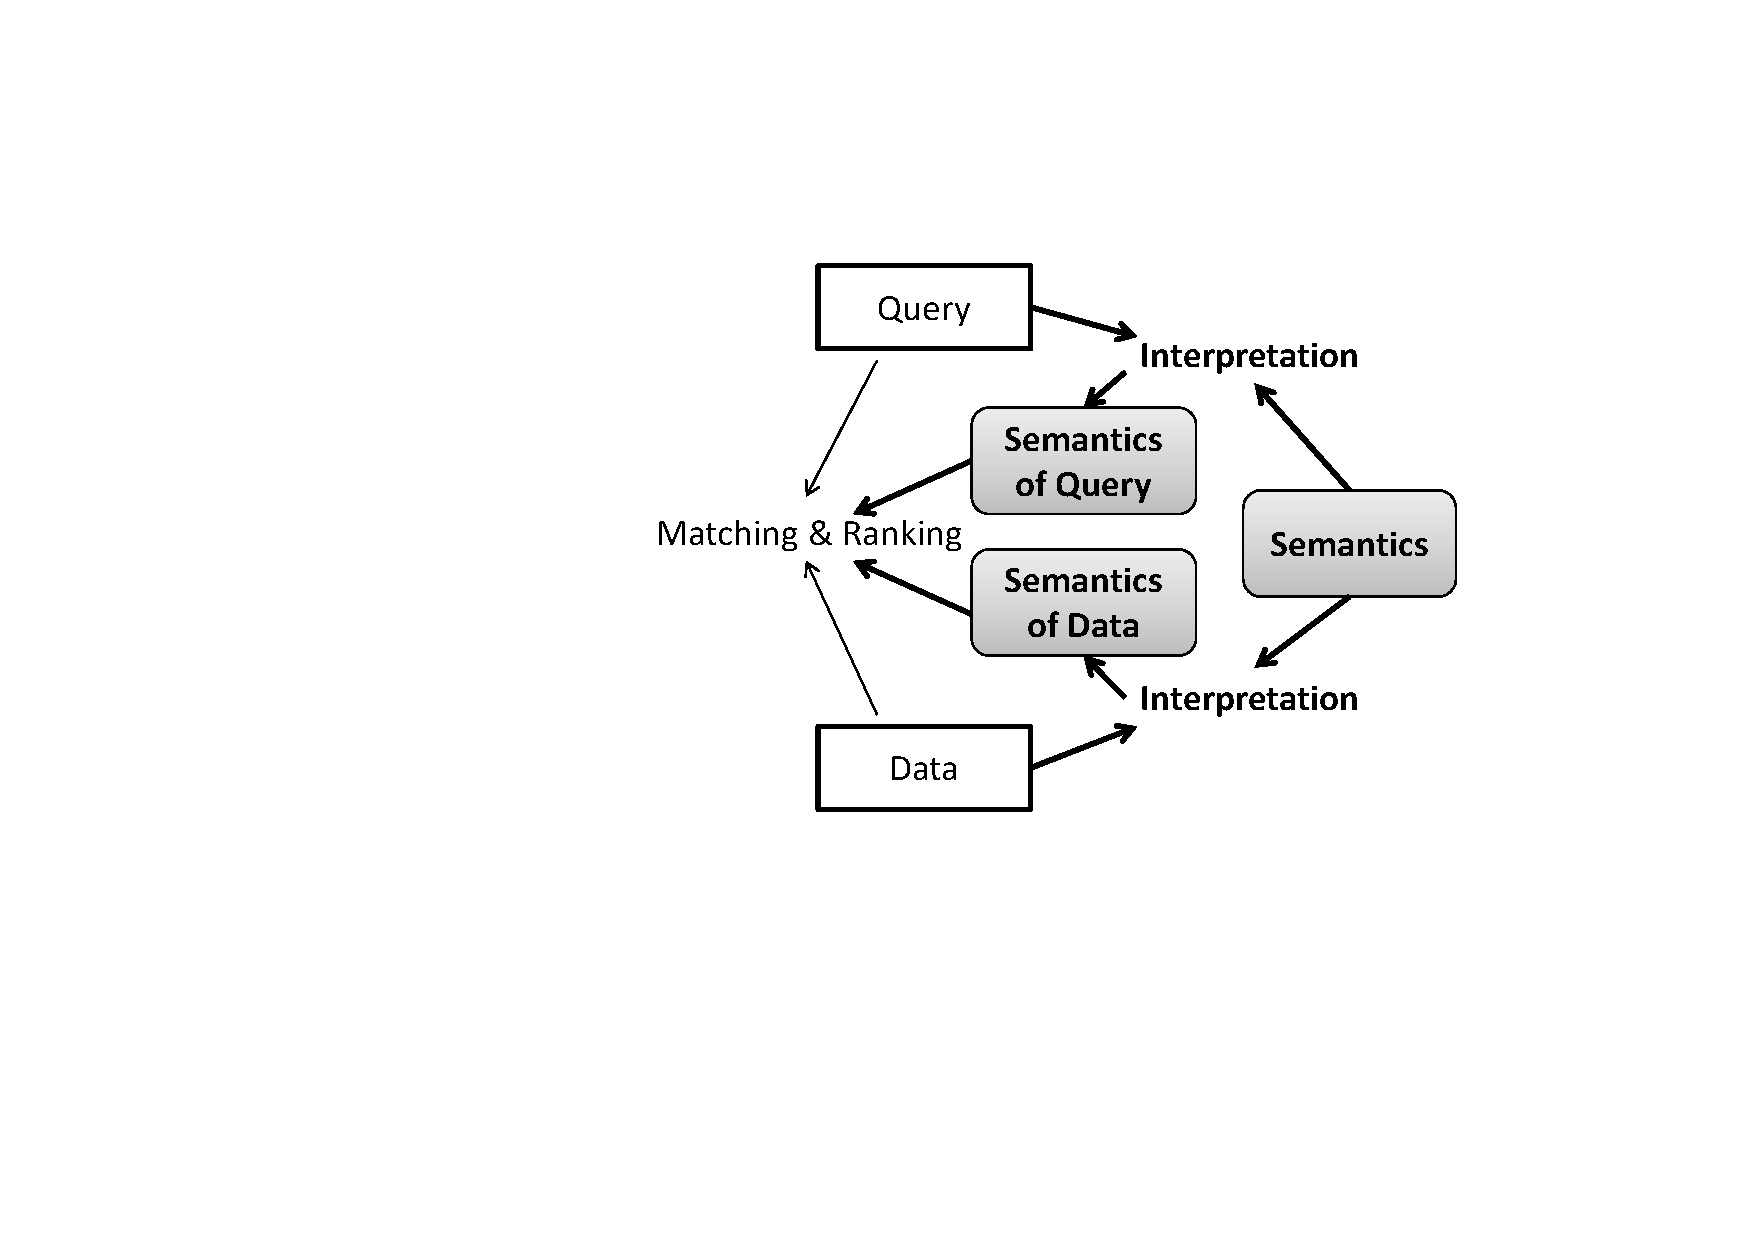
\includegraphics[width=0.35\textwidth]{figs/semsearch.pdf}
	\label{fig:semsearch}
	\caption{Semantic Search.}
\end{figure}

Basically, \emph{search} can be characterized by three components, namely the \emph{data}, the \emph{query} and the \emph{matching framework} for computing results from the data for a given query. This is illustrated in the left portion of Fig.~\ref{fig:semsearch}. One main characteristic of concepts behind search is its emphasize on \emph{end users}. That is, search typically involves intuitive interfaces targeting users, who may do not possess knowledge about the domain, the data, and the underlying query language. The query inputs that can be obtained from these interfaces are often ambiguous. That is, they allow for many possible interpretations, which in turn, result in many possible results. Because end users are often only interested in the few best results, \emph{ranking} is considered as an essential component in search. That is, the matching framework not only specifies what constitutes matches but also their degree of matching.   

\emph{Semantic search} is a concept widely used by different communities to refer to search approaches that broadly speaking, aim to \emph{use semantics to improve the search experience}. Considering the core search tasks, semantics has been used to obtain a better understanding of the data and query and to improve matching and ranking based on that (see Fig.~\ref{fig:semsearch}). There are exist different notions of semantics. One the one hand, there are proposals for using the semantics of words captured as latent concepts (e.g. to use Latent Semantic Indexing for IR \cite{DBLP:conf/sigir/Hofmann99}) or latent topics (e.g. to use Latent Dirichlet Allocation~\cite{DBLP:conf/sigir/WeiC06}). While these models only implicitly capture the semantics in terms of some latent, unknown dimensions, there are also explicit models of semantics. For instance, Explicit Semantic Analysis uses Wikipedia articles, categories, and relations between articles to capture semantics. Other explicit models of semantics (henceforth called \emph{semantic models}) include thesauri, the terminological part (TBox) of ontologies and data schemas. While these models capture semantics at the conceptual level, there are also \emph{semantic data} capturing the semantics of individual entities. To accommodate the plethora of approaches that exist, we propose the following definition of semantic search.

\begin{definition}[Semantic Search] Semantic search is a search paradigm that make uses of \emph{explicit semantics} to solve any of the \emph{core search tasks}, i.e. interpreting query and (or) data, matching and ranking. 
\end{definition}

While all existing semantic search systems use some kinds of explicit semantics, the retrieval context and the specific semantic models and data used to deal with the meaning behind the query intent and data vary. 

\emph{Document Retrieval:} The IR community targets the document retrieval context where results are to be retrieved from a collection of documents. The traditional type of semantic models used here are thesauri that are employed to \emph{interpret} the terms in the textual representation of queries and data (i.e. documents). Recently, semantic data such as RDF resource descriptions have also been employed to interpret query and documents in terms of real-world entities and their relations. 

\emph{Data Retrieval:} Querying entities and their relationships is a core problem in database research. As opposed to the hidden semantics of textual content in documents, information about entities and their relationships are explicitly available in this setting -- either directly as semantic data in RDF or as structured data that can be converted to RDF. Thus, understanding the semantics of the underlying data is not the problem here. However, as opposed to classic data retrieval that is based on structured query languages, intuitive query interfaces are needed in the search context. This lead to the classic search problems of interpreting the query intent and ranking the many possible results. 
%Just like in the document context, the goal here is to enable easy access to the most relevant results. Especially in the Semantic Web community, solutions targeting this problem are also referred to as semantic search because they use semantic data to interpret the query intent and to rank results. 

%In this section, we establish the main dimensions in which existing solutions vary and then discussed them in more detail in the subsequent sections. 
% and then, provide a taxonomy of semantic search approaches. We focus on approaches studied by researchers in the Semantic Web community that explicitly target semantic search. Selectively, we also point out works from the IR and database communities that deal with the same problem. 
%Search is about retrieving information that are relevant with respect to a given information need. 
%Generally speaking, approaches that fall under the category of \emph{semantic search} use semantic data for representing information and (or) semantic models for interpreting the data and information needs. 
We characterize the many different solutions along the following dimensions:

\begin{itemize}
\item the type of targeted \emph{information needs},  
\item the representation of the information need called \textit{query}, 
\item the representation of the underlying resources called \emph{data}, 
\item the \emph{semantic models} used to understand query and data, 
\item the framework for \emph{matching} queries against data, which also involves \emph{interpreting} the content and the user intent as well as \emph{ranking} the results.  
\end{itemize}


A general overview of the main types of information needs (results), queries, data, semantic models as well as interpretation, matching and ranking techniques supported by existing semantic search solutions is illustrated in Fig.~\ref{fig:semsearch_detailed}. We will now discuss existing solutions along these dimensions. 

\begin{figure*}[tbh]
	\centering
		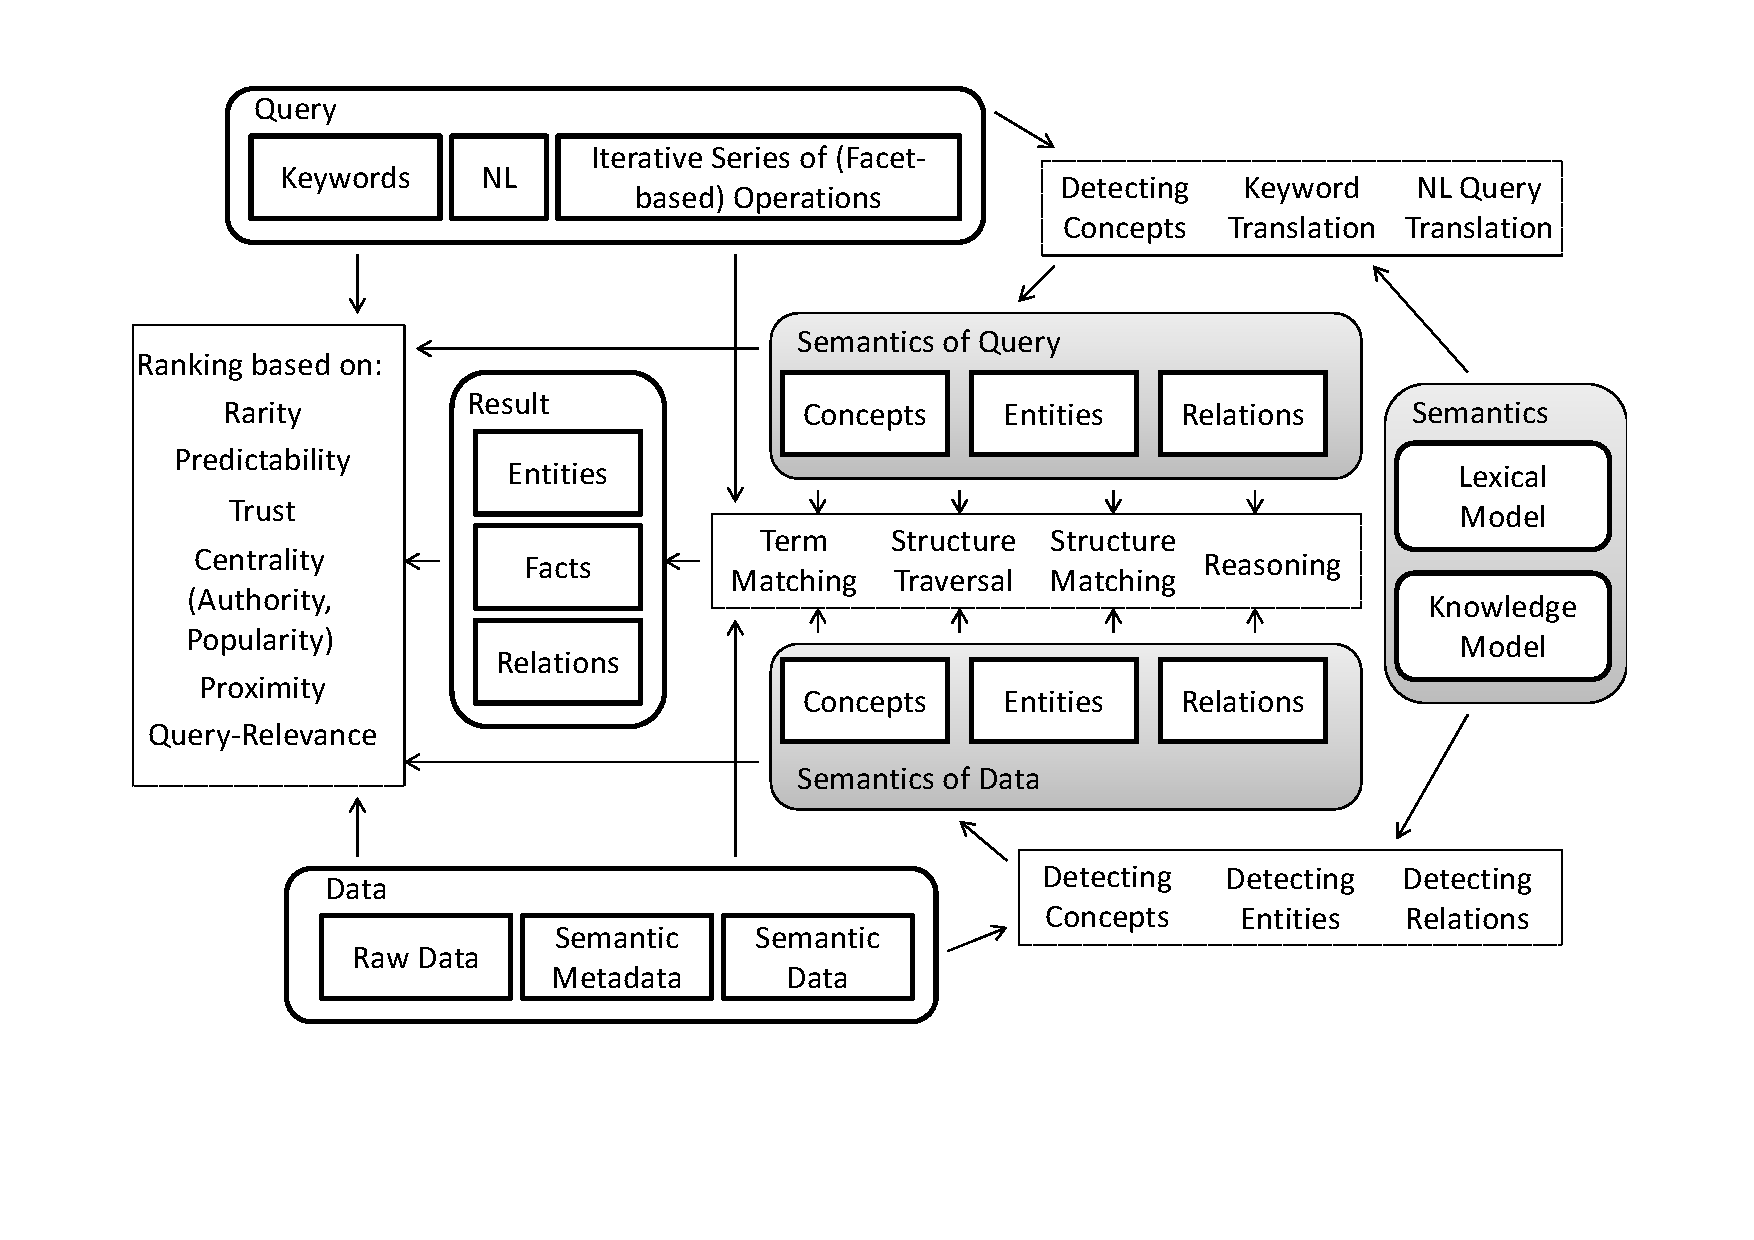
\includegraphics[width=0.85\textwidth]{figs/semsearch_detailed.pdf}
	\label{fig:semsearch_detailed}
	\caption{Overview of Semantic Search Approaches.}
\end{figure*}

\section{Information Needs}
The main motivation for semantic search is to go beyond the relatively frequent but simple queries currently supported by existing search solutions to solve the long-tail queries representing rather complex information needs. But also for simple queries, semantic data have proven to be valuable. Instead of showing documents, semantic data are used by commercial Web search engines to create rich snippets for Web pages, or to deliver direct answers. 

\subsection{Entity Search} most queries on the Web asked for Web pages representing entities such as organization or people. They are used to obtain entry points, while additional navigation and browsing is still required to satisfy the actual information need. Thus, these queries are also referred to as navigational queries. Semantic data embedded in Web pages have been exploited by Google to present rich entity snippets\footnote{Google Rich Snippets} to this kind of queries. Instead of searching over a collection of documents, semantic search engines such as Falcons~\cite{DBLP:journals/ijswis/ChengQ09} and Sig.ma~\cite{DBLP:journals/ws/TummarelloCCDDD10} use semantic data only, and return entity descriptions in RDF as results. Examples for this include the one asking for ``young scholars in Germany'' already mentioned before, or the query ``Researcher Thanh Tran'' depicted in the top left portion of Fig.~\ref{fig:matching}. Results for queries of this type comprise one or several entities. 
	 
\subsection{Factual Search} While results to the previous type of queries presented to the users are either some entity descriptions or Web pages about entities, the information needs behind this type of search require specific information from these descriptions and pages, respectively. Many searches on the Web for instance, aim at finding the ratings of restaurants, or the phone number of a particular person. To continue with our example, users may directly ask for ``the birth place of young scholars in Germany''. Direct answers to this type of queries are supported by WolframAlpha\footnote{\url{http://www.wolframalpha.com/}} and True Knowledge~\footnote{\url{http://www.trueknowledge.com/}}, or the various research prototypes such as Hermes~\cite{DBLP:journals/ws/TranWH09} or AquaLog~\cite{DBLP:journals/ws/LopezUMP07}. Since factual search is mostly about facts that correspond to attribute values of entities, it is often regarded as a particular type of entity search. We also do not further distinguish this from the general entity search task. 
 
\subsection{Relational Search} The information need here goes beyond single entities and their factual information. Answers to queries of this type comprise several entities and relationships between them. Hence, processing these queries requires some understanding of relations between entities. For instance, the example presented in the introduction about 32 year old computer scientists requires knowledge about their \verb+lives in+ and \verb+birth place+ relations to some locations. Relations may be explicitly specified as part of the keyword or NL query, and entities satisfying these relation constraints can be computed using SemSearchPro~\cite{DBLP:journals/ws/TranHL11} or AquaLog~\cite{DBLP:journals/ws/LopezUMP07}. Other systems such as NAGA~\cite{DBLP:conf/icde/KasneciSIRW08} also support searches where relations to be considered are not explicitly mentioned in the query, or unknown. They address information needs that involve finding ``how some entities are related to some other entities''. The interesting part of the results here are thus not the entities, but the relationships between them -- also referred in literatures as semantic associations (direct connection) or property sequence (path)~\cite{DBLP:conf/www/AnyanwuS03}. An example for this query, asking for paths between ``Peter Mika'' and ``Thanh Tran'' is depicted in top right portion of Fig.~\ref{fig:matching}.
	

\section{Queries}
Typically, answering complex questions requires the expertise of technical users who know the underlying data and schema and use them to formulate questions as structured queries. However, search is commonly seen as an end-user oriented paradigm, which instead of using structured query languages, involves intuitive and easy-to use access interfaces. The there main interfaces studied for semantic search are based on keywords, NL, and facets. Often, a combination of these paradigms, e.g. keywords and facets, is used to support an iterative search process where instead of constructing the query at once, the user modifies the query and results respectively, through a series of operations.    

\subsection{Keyword Search} Expressing the information needs as keywords is a paradigm that is not only popular for Web search but also widely adopted by the new breed of semantic search solutions. Most engines focusing on entity search such as Falcons~\cite{DBLP:journals/ijswis/ChengQ09} and Sig.ma~\cite{DBLP:journals/ws/TummarelloCCDDD10} feature a keyword search interface. Keywords can also be used to formulate more complex relational searches. Addressing this scenario, engines such as Hermes~\cite{DBLP:journals/ws/TranWH09}, SemSearchPro~\cite{DBLP:journals/ws/TranHL11}, AVATAR~\cite{DBLP:conf/sigmod/KandoganKRVZ06} and TASTIER~\cite{DBLP:conf/sigmod/LiJLF0} retrieve entities matching keywords, and search for relations between them in the data. 
	
	
\subsection{NL Search} This is the other paradigm for users to express their needs using their own words. Traditionally, it has been used to formulate complex questions against expert systems built for specific domains. Recently, NL interfaces have proven to be also applicable and useful for the multiple domains setting and especially for Web search -- as demonstrated by commercial engines such as WolframAlpha and True Knowledge. 	
	

\subsection{Faceted Search} Instead of formulating the entire query at once, \emph{faceted search} supports an iterative process of querying, browsing and query refinement. Upon the initial search performed by the user (e.g. using keyword search), faceted search systems~\cite{DBLP:conf/dexa/WagnerLT11,DBLP:conf/semweb/FerreH11,DBLP:conf/esws/HeimEZ10} presents results as well as facets representing attributes and relations relevant for entities in the result list. These facets can then be used to browse the results and to refine or expand the initial query. While most faceted search solutions focus on browsing and refining results of entity queries, faceted search in principle can also be used to capture complex needs. For instance, gFacet\cite{DBLP:conf/esws/HeimEZ10} supports relational search through the construction of complex facet graphs representing different types of entities and relations between them. 

\subsection{Iterative Search}
While faceted search is a popular paradigm, there are other similar interfaces that support an \emph{iterative search} process. Instead of showing facets as users type, also \emph{completions} of the user keywords as well as completions in the form of results matching the (possible interpretations of the) the keywords provided so far (also called result completion~\cite{DBLP:conf/esws/TranMH10}) have been presented. For instance, ESTER~\cite{DBLP:conf/sigir/BastCSW07} shows entity search results matching the keywords as well as their facets while TASTIER~\cite{DBLP:conf/sigmod/LiJLF09}, provides type-ahead search by finding complex (joins of) database tuples as the user types in query keywords. With these systems, users can iteratively construct the query by selecting the presented completions and facets. VisiNav~\cite{DBLP:journals/ws/Harth10} goes beyond this, allowing iterative query construction also via drag and drop. 	
	

\section{Data}
Data used in semantic search solutions can be broadly categorized into two types, namely \emph{semantic data} and \emph{raw data}. The latter basically comprises all representations of media objects such as audio, video and text. 
There are solutions~\cite{DBLP:journals/ijswis/ChengQ09,DBLP:journals/ws/TummarelloCCDDD10,DBLP:journals/ws/TranWH09}, which specifically target the data extracted from Semantic Web sources. That is, they directly operate on semantic data. In fact, structured data used in most data retrieval systems can be converted to a form that corresponds to the general notion of semantic data~\cite{DBLP:conf/sigmod/LiJLF09}. On the other hand, semantics may not be directly captured by semantic data but extracted from raw data. This is especially the case for document retrieval systems, where one of the essential task in semantic search is to obtain a semantic data representation of the documents (called \emph{semantic metadata}). 


\subsection{Structured / Semantic Data}  The most common type of semantic data used in semantic search systems is RDF. Basically, RDF can be seen as a graph-structured model, representing entities, their attributes, and relations between them as a set of triples. A visual representation of such a \emph{semantic data graph} capturing information about two \verb+researcher+s with the \verb+name+s \verb+Thanh Tran+ and \verb+Peter Mika+ is depicted in the bottom portion of Fig.~\ref{fig:matching} 

This general graph-structured model can be used to capture structured data of different types. In fact, most of the data made publicly available on the Web and incorporated into semantic search engines such as Falcons~\cite{DBLP:journals/ijswis/ChengQ09}, Sig.ma~\cite{DBLP:journals/ws/TummarelloCCDDD10} and Hermes~\cite{DBLP:journals/ws/TranWH09} originate from relational or XML databases. XML elements can be represented as nodes, and their structure information can be captured as edges. Likewise, information contained in tuples of a relation database can be mapped to nodes, while foreign key relationships can be modeled as edges. In fact, the conversion of XML and relational data to a RDF semantic data graph can be accomplished by using mapping rules, and there exist many standards and tools for accomplishing that (see \url{http://www.w3.org/2001/sw/rdb2rdf/}).  Represented as RDF, these and possibly other types of structured data also capture knowledge in terms of entities and their relations. Hence, especially after its conversion to RDF, structured data is often synonymously referred to as semantic data. In line with this general notion, semantic data used in semantic search systems can be defined as follows:

\begin{definition}[Semantic Data] 
Semantic data can be conceived as a graph, where nodes represent \emph{entities} and their \emph{attribute values}, and edges stand for \emph{attributes} of entities or \emph{relations} between entities. 
\end{definition}

Besides the various RDF datasets that exist on the Web, such as the hundreds of heterogeneous sources that have been made available as Linked Data~\footnote{\url{http://linkeddata.org/}}, Wikipedia can be as an extreme example that lies at one end of the spectrum of semantic data. While it is actually a collection of documents (i.e. contains mainly textual data), it fits the presented notion of semantic data because every Wikipedia page corresponds to an entity, and there are links between Wikipedia pages that can be seen as relations. In fact, exploiting this and other specific features of Wikipedia articles such as Infoboxes, a RDF dataset called DBpedia~\cite{DBLP:journals/ws/BizerLKABCH09} has been automatically derived from this collection. Wikipedia as a source of semantics is particularly popular for search systems that focus on expert search or entity search in general. It is used either to directly answer entity search queries, or as background knowledge~\cite{DBLP:conf/cikm/KapteinSVK10,DBLP:conf/cikm/BronBR10}. 

On the other end of the spectrum, there are more formal views on what constitute semantic data. In particular, many researchers may argue that the reason why RDF, and other data models that are built upon a formal model of semantics, are actually called semantic data (instead of structured data) is because they can be exploited by a reasoning engine to infer new knowledge (i.e. the knowledge that is entailed by the semantics). While the formal model of semantics specified for RDF is relatively simple (consists of a few inference rules), semantic data used in existing search systems have also been represented using more expressive knowledge representation languages such as OWL and F-logic. For instance, Serene~\cite{DBLP:journals/ws/FazzingaGGL11} makes use of facts that are captured as Abox assertions of an OWL ontology, while ORAKEL~\cite{DBLP:journals/dke/CimianoHHMS08} search over an F-logic knowledge base. However, while the use of formal semantics and reasoning has been investigated, they play only a limited role in existing systems. The 
majority of approaches does not rely on reasoning. It seems that the research focus still lies in correctly understanding the ambiguous queries and data (namely, to interpret queries and data as elements of the semantic data model as defined above), while reasoning over semantic data is beneficial but not essential yet. 

Accordingly, a general notion of semantic data is employed in this work to consider all those systems, which consider the semantics of entities and relations but may not have a formal model of semantics available, or does not exploit it for search. 
	
\begin{figure}[thb]
	\centering
		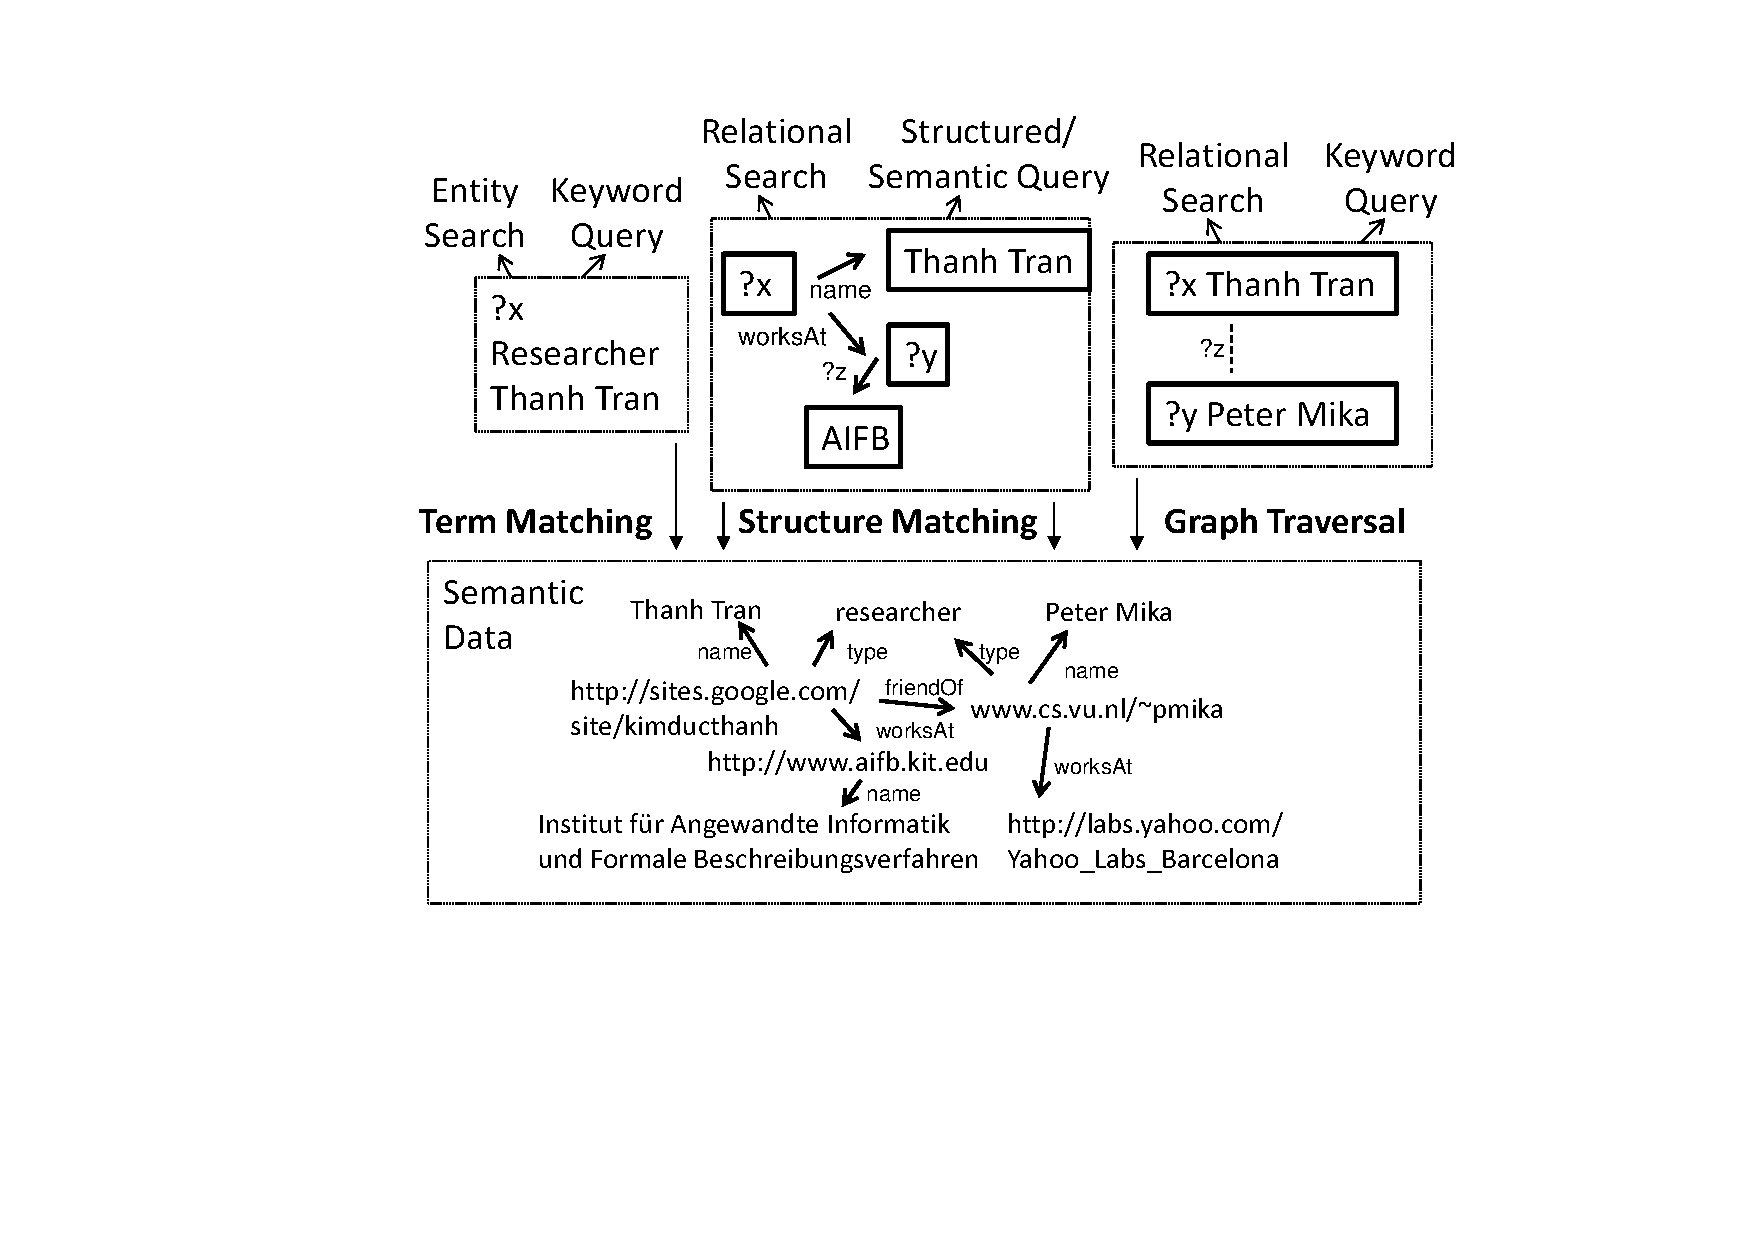
\includegraphics[width=0.5\textwidth]{figs/matching.pdf}
	\label{fig:matching}
	\caption{Examples for semantic data, queries and matching techniques.}
\end{figure}
	
\subsection{Raw Data and Semantic Metadata} There are engines directly operating on semantic data to provide direct answers (data retrieval systems). These are mainly systems, which provide search interfaces over structured databases that have been converted to semantic data graphs~\cite{DBLP:conf/sigmod/LiJLF09,DBLP:conf/sigmod/LiOFWZ08}, or RDF data and ontologies crawled from the Semantic web~\cite{DBLP:journals/ijswis/ChengQ09,DBLP:journals/ws/TranWH09,DBLP:journals/ws/HoganHUKPD11}. Besides them, there are also semantic search systems supporting the retrieval of documents or media objects in general. They employ semantic metadata, often in combination with the raw data representation of these objects. Basically, semantic metadata is semantic data that captures information about the objects to be retrieved. Because it is clear from the context, these terms are often used synonymously (in this work). Metadata includes basic information about the objects such as \verb+author+ and \verb+year+. One main challenge in semantic search is to interpret the semantics behind the content captured as raw data and to represent it as semantic metadata. For instance, the content of a document may be recognized as referring to a \verb+meeting+ with the two \verb+researcher+s \verb+Peter Mika+ and \verb+Thanh Tran+ as \verb+participant+s. Semantic metadata representing the content may also be manually produced and embedded into the objects. Recently, several industry projects such as Google Rich Snippets and Yahoo! SearchMonkey actively target this development, providing incentives for site owners to embed RDFa or other kind of semantic metadata into their Web pages. Note that while we discussed how to conceive Wikipedia as semantic data (with pages corresponding to entities), a more typical viewpoint is to consider it as a collection of documents that are manually associated with metadata: every page is associated with a set of categories and exactly one entity (the entity it is about).  

While the amount of available metadata is increasing, it is still too sparse to cover all information needs. Thus, metadata is mostly used as additional information that can help to improve standard search over raw data~\cite{DBLP:journals/tkde/CastellsFV07,DBLP:journals/ws/FernandezCLVCM11}. Search over raw data can also be seen as a fall-back solution for cases where metadata cannot completely satisfy the information need. There exists also proposals for ontology-based IR, which completely rely on metadata~\cite{tran2007expressive}. In this case the retrieval of documents is formulated as a data retrieval task, where data about the documents (metadata) is returned as a direct answer. 


\section{Semantics \& Semantic Models}
\begin{figure}[thb]
	\centering
		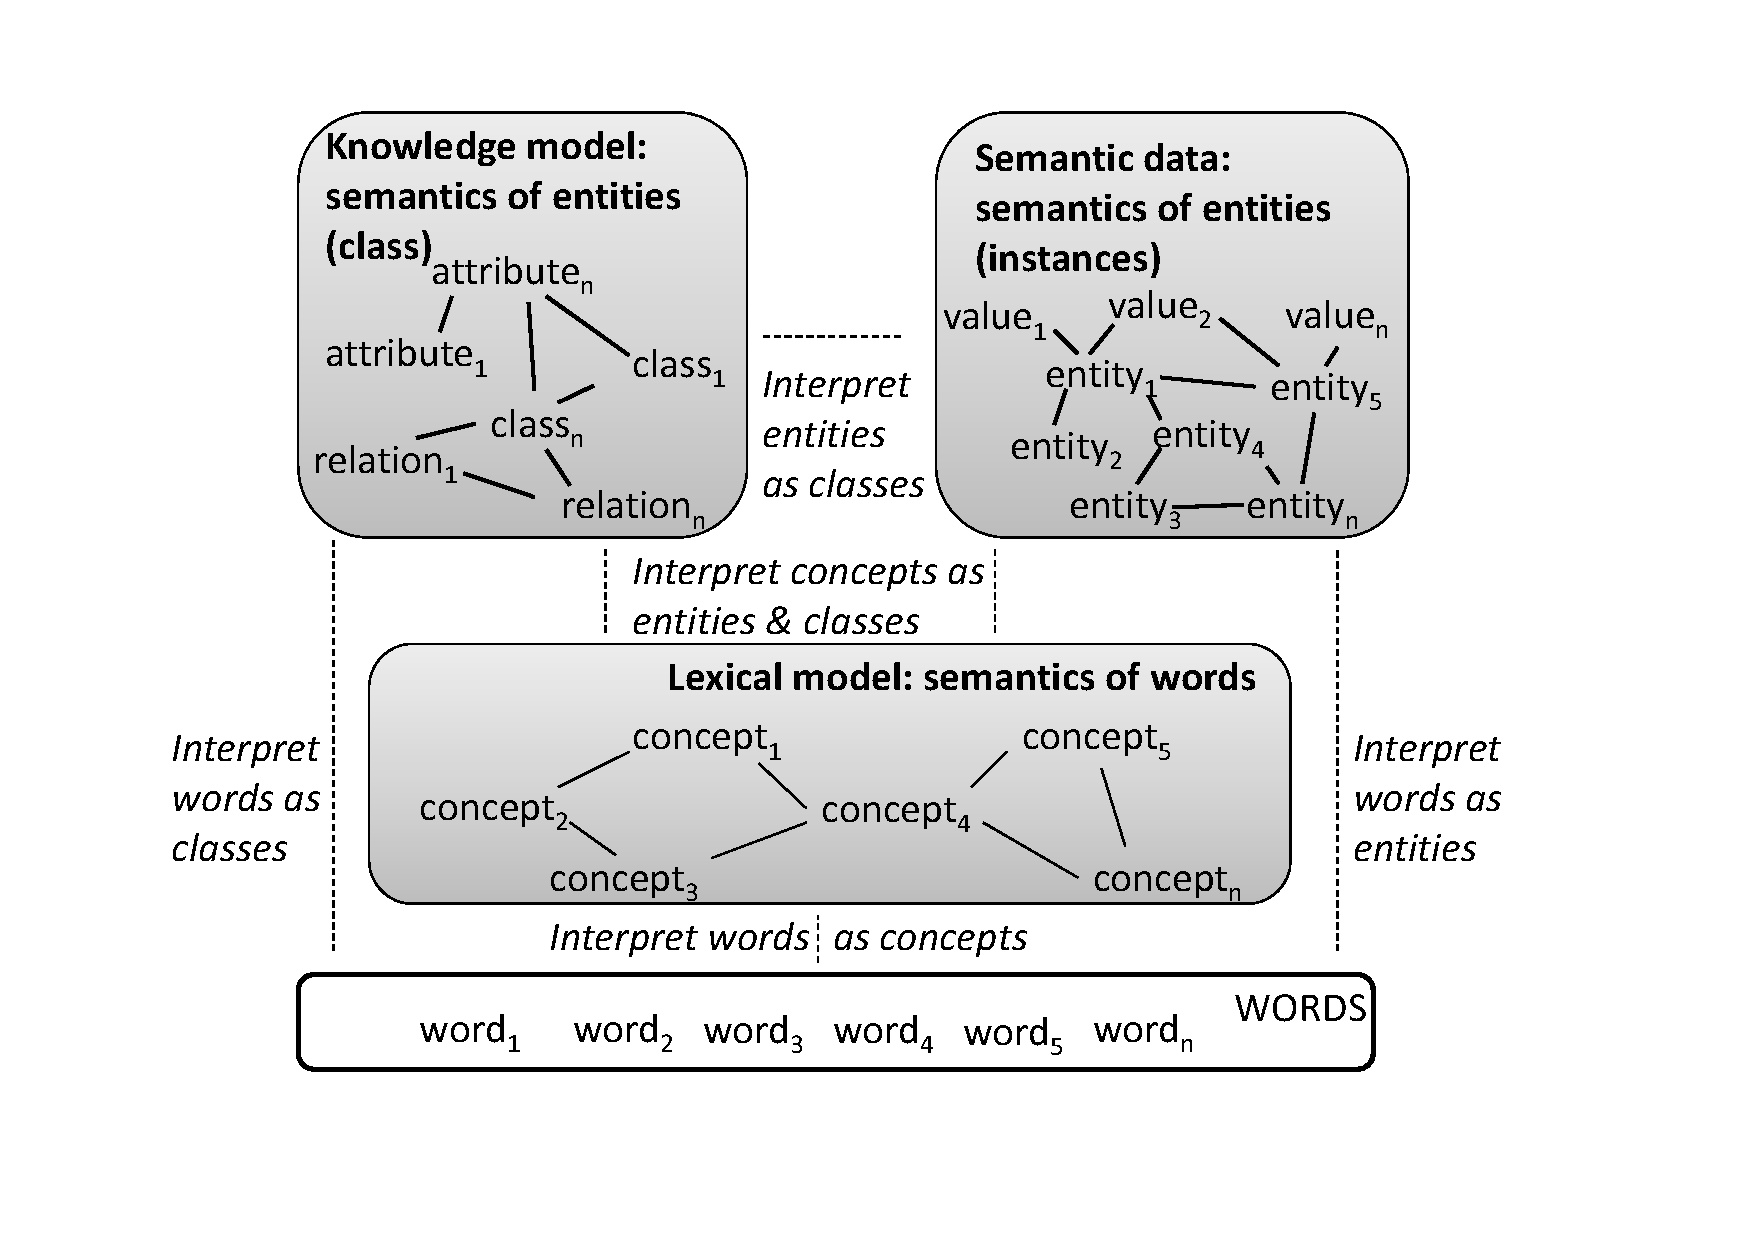
\includegraphics[width=0.5\textwidth]{figs/semantic_layer.pdf}
	\label{fig:semantic_layer}
	\caption{Words, concepts and entities.}
\end{figure}

As discussed, central to semantic search system is the use of semantics. A main source of semantics is the semantic data itself. This semantics of entities is illustrated in the top right corner of Fig.~\ref{fig:semantic_layer}. Additionally, this figure also shows additional sources of semantics as well as their use in the semantic search context, namely to understand words in terms of concepts and entities. Broadly, \emph{lexical models}, which capture semantics at the level of words in terms of \emph{concepts}, can be distinguished from \emph{knowledge models}, which capture real-world knowledge in terms of \emph{entities}, \emph{classes}, \emph{relations}, and \emph{attributes}.  

\subsection{Knowledge Models} While semantic data capture concrete entities (instances), these are abstract models of knowledge, basically representing classes of entities, attributes associated with these classes, and relations between classes. This is visualized in the top left portion of Fig.~\ref{fig:semantic_layer}.  

Different models, which vary in the degree of formality and expressiveness have been used by different communities for semantic search. The model used in ORAKEL for NL question answering for instance is captured by the TBox portion of an ontology and consists of classes (also called concepts) that are ordered in a subsumption hierarchy and are connected through relations. Range and domain information are captured as restrictions on the relations. As shown for Serene~\cite{DBLP:journals/ws/FazzingaGGL11}, more complex expressions can be added to capture the semantics of concepts to reflect either general knowledge (such as the knowledge encoded in Wikipedia)
or specific knowledge of a domain. Because the ontology models used in these systems are represented using the logic-based formalisms F-Logic or OWL (description logic), they can be seen as \emph{logical theories} with well-defined formal semantics. 

Also, \emph{conceptual graphs} (CGs) have been employed for representing ontology models, and used for the tasks of NL questions interpretation and answering~\cite{DBLP:conf/aswc/CaoCT08} as well as for interpreting and representing documents~\cite{DBLP:conf/iccs/ComparotHH07}. CGs combine the intuitiveness of graph-based languages and the formal foundation of logics, enabling the modeling of knowledge in terms of concepts and their relations and its mapping to different formal languages. Corese~\cite{DBLP:conf/ecai/CorbyDF04} uses CGs as an internal model (to take advantage of previous work on CGs in the KR community), which however, is translated to RDFS to conform with this more commonly used standard language for representing RDF schemas. 

Closer to the end of linguistic models discussed next are knowledge models that consist of concepts only. For instance, C-Search encodes knowledge as concepts expressed in propositional description logic (DL). This DL does not feature the representation of relations (also called roles) but the specification of complex concepts as a conjunction or disjunction of atomic concepts. 

		
\subsection{Lexical Models} The use of concepts has already been investigated in the early years of IR research~\cite{DBLP:conf/sigir/Giger88}. Different to knowledge models, which capture semantics in terms of real-world entities and their relations, the models employed there are lexical in that they capture semantics at the level of words. While concepts in knowledge models stand for classes of real-world entities, concepts in lexical models correspond to \emph{senses of words}. The latter are more general such that they may refer to entities, classes, relations, attributes, or other senses of words. While these different ``types'' of senses are not explicitly distinguished, concepts are organized along lexical relationships in a lexical model. 

\emph{Thesaurus} (often, \emph{lexicon} is also used as synonym) is a popular lexical model that has been extensively used for document retrieval in IR, which basically, groups words together according to their semantic similarity. Each group represents a different word sense. In practice, lexical databases also considered as thesauri such as WordNet, or thesauri used in classic IR systems~\cite{DBLP:conf/sigir/Giger88}, not only capture senses (concepts) and their lexical variants, but also relationships between them such as synonym, broader, narrower and related. This is illustrated in the bottom part of Fig.~\ref{fig:semantic_layer}. 


\subsection{Semantics} 
Based on the above discussion, we derive a general notion of semantics that is used to characterize the different types of semantic search systems.

\begin{definition}[Semantics] 
The semantics of queries and data are captured by semantic search systems in different ways. Semantics can be represented (1) as word senses that are organized through lexical relations between words (\emph{lexical model}), (2) as specific knowledge about concrete entities, i.e. specific attribute values and individual relations between entities (\emph{semantic data}) or (3) as general knowledge about classes of entities, their attributes, and relations between classes (\emph{knowledge model}). 
\end{definition}

A prominent example that can be used to illustrate these many aspects of semantics is Wikipedia. As discussed, it has been used as semantic data to answer entity search queries, and converted to a semantic dataset called DBpedia. The Wikipedia categories of pages have been treated as classes and used to construct hierarchies of classes in an ontology called YAGO~\cite{DBLP:conf/www/SuchanekKW07}. Wikipedia is also used as a source for Explicit Semantic Analysis (ESA), where every Wikipedia page is regarded as a concept. Because ESA does not distinguish entities and classes, the concepts here can be seen as word senses. Thus, Wikipedia pages and links constitute a lexical model in this context. 

\subsection{Focus: Semantics of Entities \& Relations} 

The discussion of semantics so far focuses on entities and simply (binary) relations between them. Yet, the kind of semantics that can be expressed is only limited by the knowledge representation (KR) languages. There exist very powerful KR formalisms and many of them have been incorporated to perform document retrieval (already in the early years of IR~\cite{DBLP:conf/sigir/Rijsbergen89}) and to represent complex queries and knowledge used in NL question answering~\cite{DBLP:journals/tkde/VassiliadisTK94}(in the early years of expert systems). For instance, the employed formalisms have been used to represent temporal or fuzzy aspects of world knowledge. However, there are practical reasons why the focus of current research (and this paper) is set on simple descriptions of entities. On the hand, most queries on the Web seem to ask about entities and their relations. That is, most common queries as well as a large part of queries in the long tail (of Web query logs) are about entities and their relations (i.e., they are of the types entity, factual or relational queries). More importantly, the bottleneck is actually the availability of data. It became evident that manually capturing the content of documents as complex logical formulas does not scale. Extracting entities and relations from documents at high quality still remain hard problems, representing the limits of what can be done automatically by data extraction technologies. Also, most of the data residing in databases nowadays are mainly about entities and their relations. \dtr{maybe also discuss the difference to XML retrieval, which merely use structure information for ``focused'' retrieval: retrieve components of the structured XML documents that match the query}

 
\section{Interpretation}

\subsection{Content Interpretation} 
	
One crucial task in supporting semantic search over documents is to obtain a richer understanding and representation of the document collection. Instead of a the typical bag-of-words model used in classic IR, the goal is to capture the content of the documents as entities, concepts and relations, i.e. as semantic data or elements of a semantic model. For this, different tools for Natural Language Processing (NLP) have been employed. 

\emph{Detecting Concepts:} Documents have been analyzed to extract concepts for the task of modeling documents as conceptual graphs~\cite{DBLP:conf/iccs/ComparotHH07}. For C-Search~\cite{DBLP:conf/esws/GiunchigliaKZ09}, which represent documents as DL concepts corresponding to WordNet senses, the authors identify words in documents matching senses, and uses POS tagging information and lexical database to perform word sense disambiguation. While words are mapped to atomic concepts, phrases are represented as complex concepts using DL formulas~\cite{DBLP:conf/esws/GiunchigliaKZ09}. Especially in the biomedical domain, the use of thesauri concepts for interpreting and representing documents is very common~\cite{DBLP:conf/trec/TrieschniggKS06,DBLP:conf/trec/ZhouYTS06}. For instance, the Unified Medical Language System and a gene-thesaurus have been used to identify multi-word terms and to map synonymous words to one concept~\cite{DBLP:conf/trec/TrieschniggKS06}. The concepts were identified simply by by comparing document words to thesaurus terms.
	
\emph{Detecting Entities \& Relations}: For extracting entities and relations, the large body of research work on named entity recognition and data extraction has been leveraged by existing semantic search solutions. One of the platform, which is most frequently used by semantic search systems for extracting semantic data and
automatically annotating document collections at a large scale is KIM~\cite{KIM DBLP:journals/ws/KiryakovPTMO04}. IBM's AVATAR~\cite{DBLP:conf/sigmod/KandoganKRVZ06} makes use of UIMA, a framework of annotators that can be configured in a pipeline to analyze and extract data from text. There is a another work from IBM, which focuses on extracting named entities and relations from text and using them for more precise search~\cite{DBLP:conf/sigir/Chu-CarrollPCFD06,DBLP:conf/cikm/Chu-CarrollP07}. Also for this task, lexical resources, particularly Gazetteers, is frequently used. For disambiguating named entities mentions in text, it has been shown that semantic data about entities and their relations provides valuable information~\cite{DBLP:conf/esws/KlebA10}. The technique behind this is based on graph traversal, which starts from nodes matching the entity mentions. Controlled through spreading activation, path from these nodes are traversed to explore the semantic context of these nodes (i.e. entities). These contextual interpretations are then used for disambiguation. A special case of understand


\subsection{Query Interpretation} 
	Essentially, interpreting queries is similar to the task of understanding text in documents. The difference is that instead besides NL text, also keywords may be provided as inputs. 
	
\emph{Translating NL Queries:} Names entities, their types and relations between them are identified from NL questions~\cite{DBLP:conf/aswc/CaoCT08} and used to construct a semantic representation of the information need, i.e. a \emph{structure/semantic query}. Analogous to structured/semantic data, there is no clear distinction between a structured query and a semantic query (and thus, the corresponding terms are also used as synonyms). Basically, they capture the information need in terms of entities, their relations and variables that represent existential quantifiers or the pieces of information to be retrieved. While the common language used to query RDF is SPARQL, other (logic-based) formalisms have been used. Besides conceptual graphs~\cite{DBLP:conf/aswc/CaoCT08}, recognized entities, types and relations are also represented as logical formulas~\cite{DBLP:journals/dke/CimianoHHMS08}, XML Fragments~\cite{DBLP:conf/sigir/Chu-CarrollPCFD06} or SPARQL queries~\cite{DBLP:conf/esws/DamljanovicAC10}. For processing NL questions, the same NLP tools used for content interpretation have been applied. For instance, the Stanford Parser~\footnote{\url{http://nlp.stanford.edu/software/lex-parser.shtml}} and GATE~\footnote{\url{http://gate.ac.uk/}} are used by FREyA~\cite{DBLP:conf/esws/DamljanovicAC10} to obtain the syntactic parse tree and to identify concepts in NL questions, respectively. Besides the semantic data or additional semantic models such as a domain ontology, lexicons specifying the mappings between syntactic elements,
such as verbs or nouns with their arguments identified by the parser, and concepts and relations in the semantic models, have been used for NL question answering~\cite{DBLP:journals/dke/CimianoHHMS08}. This is to deal with the fact that these semantic elements have many lexical variants. These mappings are specified by lexicon engineers. Such a lexicon is especially needed for porting the NL interface from one domain to one other. Aiming at reducing this upfront customization effort and domain independence, there are also systems that in the case of lexical ambiguities, ask users to provide mappings, and use them to train models (e.g. via reinforcement learning~\cite{DBLP:conf/esws/DamljanovicAC10}) that automatically compute mappings. While it has been reported~\cite{DBLP:journals/ws/LopezUMP07} that domain customization usually improves recall, many NL-based semantic search systems exploit general domain-independent lexical resources (e.g. WordNet is used by AquaLog~\cite{DBLP:journals/ws/LopezUMP07}) but do not require domain-specific lexicons.

	\emph{Detecting Concepts in Keyword Queries:} One of the main challenge in dealing with keywords in queries or NL words in general is their semantic ambiguity. The same meaning can be expressed in different ways. In particular, there are lexical variants that refer to the same concept, relation or entity (synonymy). One and the same word however, can also have different meanings (polysemy). These are only two prominent problems, and there exist many other subtle ambiguities (e.g. terms overlap or are related in meaning). The use of thesaurus (also called lexicon) to deal with semantic ambiguities of words has long history and has been investigated as the problem of concept-based IR~\cite{DBLP:conf/sigir/Giger88}. Concept-based IR is especially needed in the biomedical domain due to the frequent presence of acronyms, homonyms and synonyms. For detecting the underlying concepts, many lexical resources that are abundantly available for this domain, such as the Online Dictionary of Abbreviations from MEDLINE, the MESH thesaurus and the Gene Ontology have been used~\cite{DBLP:conf/sigir/ZhongH06,DBLP:conf/trec/JelierSEWMSMK03}. The detected concepts are used to expand the query~\cite{DBLP:conf/sigir/QiuF93,DBLP:conf/trec/JelierSEWMSMK03}. Concept-based query expansion \cite{DBLP:conf/sigir/QiuF93} for instance, detect the concept behind the query, and perform selection and weighting of additional search terms directly based on this concept (instead of the query terms). This and other works in this era, were based on the use of thesauri that capture concepts and relationships. WordNet for instance, was use to represent concepts by WordNet synonym sets, and for expanding query terms by following WordNet links \cite{DBLP:conf/sigir/Voorhees93}. WordNet links (is-a in particular) was also used to disambiguate query terms and to choose their senses \cite{DBLP:conf/sigir/Voorhees94}. Recently, a technique based on the idea of relevance model has been proposed to recognize the concepts underlying the query, referred to as conceptual query modeling~\cite{DBLP:journals/ipm/MeijTRK10}. Instead of detecting the concepts based on a thesauri, this approach retrieves the top pseudo-relevance feedback documents through an initial query run. Concept annotations associated with these documents are then used to construct the conceptual representation of the relevance model (the query). While OntoSearch~\cite{DBLP:conf/aaai/JiangT06} does not explicitly the query and the underlying relevance, it follows a similar idea. Concepts captured by ontologies (seen as network of concepts) are used here.  First, OntoSearch obtains a set of documents for the given query, then uses the concepts associated with these documents as the seeds to the semantic network. Through spreading activation, concepts that are semantically related to this initial concept set are inferred, and used to re-rank the documents. 
	
\emph{Translating Keyword Queries:} Instead of concept-based query expansion or aiming at a conceptual representation, there are also proposals for mapping keyword queries to fully structured queries. Entities and relations in the semantic data that are mentioned in the queries are identified and represented as XML Fragments~\cite{DBLP:conf/sigir/Chu-CarrollPCFD06}. AVATAR~\cite{DBLP:conf/sigmod/KandoganKRVZ06} is another system, which supports this kind of keyword query interpretation. It maintains a translation index, which can be conceived as a lexicon that returns all meanings for an individual keyword. Specifically, it returns schema concepts as well as schema paths matching the keywords. These keyword matches are then combined to enumerate all possible interpretations of the query. For RDF data, a top-k graph traversal algorithm has been proposed to efficiently compute all possible interpretations~\cite{DBLP:conf/icde/TranWRC09}. Here, keywords are interpreted as entities, classes or relations (called keyword matching elements), which are captured by the semantic data or the underlying semantic model. All possible paths between these keyword matching elements are computed online by traversing a combination of the semantic data graph and the schema graph (the semantic model), and combined to obtain interpretations which cover all the query keywords. This keyword query interpretation is implemented by Hermes~\cite{DBLP:journals/ws/TranWH09}, and later, SemSearchPro~\cite{DBLP:journals/ws/TranHL11}. TASTIER~\cite{DBLP:conf/sigmod/LiJLF09} also applies this graph traversal mechanism to interpret keywords not as possible queries (i.e. as information needs) but as answers. As the user types, TASTIER completes the query with answers that possibly match the intended information need. 

These mentioned approaches deal with the interpretation of ambiguous queries that are expressed as NL or keywords. The end result is a more precise understanding of the need, represented as structured queries. This is also the aim of other related work that falls into the general category of query construction. For instance, faceted search~\cite{DBLP:conf/dexa/WagnerLT11,DBLP:conf/esws/HeimEZ10,DBLP:conf/semweb/FerreH11} or the other kind of iterative query interfaces based on visual manipulation (drag and drop)~\cite{DBLP:journals/ws/Harth10} as mentioned before, also belong to this general category. In these interfaces, every user operation is directly mapped to a query construct. For instance, adding and removing facets result in the addition (query expansion) and removal (query refinement) of query predicates, respectively. Clearly, the difference to work on query interpretation is the lack of ambiguity, i.e. the semantics of every user input is clear. 
	
\section{Matching}
The differences between term matching, structure matching and graph traversal are illustrated in Fig.~\ref{fig:matching}. 
	
\subsection{Term Matching} 
%\subsubsection{Term- / Content-based Matching}
This matching is needed when the representation of query and data is based on terms (i.e. is a bag of words). This is the case with all the existing concept-based document retrieval solutions~\cite{DBLP:conf/sigir/Giger88,DBLP:conf/sigir/ZhongH06,DBLP:conf/trec/JelierSEWMSMK03,DBLP:conf/sigir/QiuF93,DBLP:conf/sigir/QiuF93,DBLP:conf/sigir/Voorhees93,DBLP:conf/sigir/Voorhees94,DBLP:journals/ipm/MeijTRK10}, which identify the concepts behind the query and content but however, only use them for query or document expansion (i.e. expand the term-based query / content representation with additional terms corresponding to the identified concepts). Likewise, there are approaches, which interpret the query as entities and relations and to use this understanding to expand the queries with corresponding terms~\cite{DBLP:series/sci/NgoC10}. Many semantic data retrieval systems such as Falcons~\cite{DBLP:journals/ijswis/ChengQ09} and Sig.ma~\cite{DBLP:journals/ws/TummarelloCCDDD10} also employ bag-of-words representations -- both of the query and the semantic data. In these cases, the structure and semantics are not taken into account during the matching (but possibly, might have been used in other steps such as query interpretation). The matching boils down to the standard IR retrieval problem. Namely, given a set of keywords, documents matching individual keywords are retrieved. Typically, they are then joined to obtain those, which match all query keywords (AND-semantics). 
%This matching goes beyond the term-level to consider the content, which may contain several mentions of the query terms, as well as mentions of terms that do not appear in the query. At this content level, results may differ in the degree of matching, an aspect that is dealt with during the ranking. 

\subsection{Structure / Semantic Matching} 
	This matching is possible when the query and content are interpreted or are directly available as a structured query and semantic data, respectively. That is, the semantics of both the query and data is represented in terms of some entities and their relations. 
		
	\emph{Matching Complete Structure Patterns (Structure Matching):} Most frequent is the combination SPARQL queries and RDF data. In particular, the three common types of information needs discussed previously can be captured through the basic graph pattern (BGP) feature of SPARQL. Just like semantic data, a BGP forms a graph where nodes and edges are either constants or variables. They form complete patterns in the sense that through explicitly captured join variables, the query engines know how to combine intermediate results obtained for subparts of the queries (for triple patterns in the BGP) to compute end results. Matching BGPs against semantic data boils down to the task of \emph{graph pattern matching} where constants in the BGP representing entities, relations, attributes and attribute values are matched against the RDF data graph to find matching subgraphs that contain bindings to variables in the BGP. Processing these BGPs involves standard \emph{database query evaluation} techniques, i.e. precompile the query to capture an optimal evaluation plan, then \emph{retrieve} data (from optimized indexes) for each triple pattern and \emph{join} intermediate results according to the plan. This matching is supported by off-the-shelf triple stores. For instance, it is used by SemSearchPro~\cite{DBLP:journals/ws/TranHL11} for computing results for SPARQL queries, after they have been derived from keywords through query interpretation. 
	
	\emph{Matching Incomplete Structure Patterns (Graph Traversal):}  While join-based evaluation is possible for structured pattern that are complete, traversing the data graph is needed when query patterns entail missing connections. That is, the query engines cannot directly combine partial results based on join variables but needs to explore for different paths between them. One combination that involves this type of matching is the evaluation of keyword queries over semantic data. As discussed before, the structure and semantics in the data can be used to interpret the keyword query and to convert it to a structured query. Instead of query interpretation, there are also systems~\cite{DBLP:conf/cikm/LadwigT11,DBLP:conf/sigmod/LiOFWZ08}, which use the same \emph{graph traversal} mechanism to directly evaluate the keyword query. They skip the computation of queries and directly explore for results in the data (subgraphs) that match the keywords. As opposed to standard IR-style keyword search on documents, the results here are semantic data graphs. That is, the keywords in the query do not refer to single documents but possibly, several entities that are connected through paths in the semantic data graph. Hence, simply joining results (documents), which match the query keywords is not sufficient. Entities matching keyword(s) in the query have to be retrieved, and subgraphs containing paths, which connect these keyword matching entities have to be explored in the data through traversing graph nodes and edges. A different semantics has been used~\cite{DBLP:conf/www/RochaSA04}, where results do not have to cover those nodes matching the query keywords. Those parts of the data, which are interesting and thus, shall be explored and returned as results, are controlled through manually defined traversal constraints that are realized via spreading activation. 

Interestingly, graph traversal is also employed for the relational search scenario, where the relations (paths) between entities are unknown. For instance, the mechanism used by for graph exploration by Hermes~\cite{DBLP:journals/ws/TranWH09,DBLP:conf/icde/TranWRC09}, a keyword search system, is similar to the one proposed for answering P-Queries~\cite{DBLP:conf/www/AnyanwuS03}, a special type of queries that ask for unknown semantic associations between entities. 

Another application of graph traversal has been proposed for the combined scenario of document and data retrieval. The goal is to find entities in the knowledge base, which are related to the documents to be retrieved, or vice versa, to retrieve documents related to some given entities. The starting points here are thus documents or entities, and traversal from these points are controlled through spreading activation~\cite{DBLP:conf/esws/SchumacherSS08}.


	\emph{Reasoning:} The formal well-defined semantics of some semantics models such as ontologies represented in OWL, have also be exploited for matching. More precisely, they are used for \emph{reasoning} to consider not only the available data but also new facts that can be automatically inferred from the formal semantics. For instance, the semantic models used in Serene~\cite{DBLP:journals/ws/FazzingaGGL11} is an ontology TBox represented as DL formulas, and semantic data are captured as ABox assertions of the same ontology. Serene uses an inference engine to derive new knowledge during an offline ontology compilation step. This computation is performed offline to improve the efficiency of online matching. Clearly, new knowledge relevant for the query can also be derived online. In ORAKEL for instance, the inference of new facts is performed as part of the computation of query matches. Notably, the first system created in the early years of Semantic Web research, which makes use of logical reasoning for computing semantic matches is SHOE~\cite{DBLP:conf/dagstuhl/HeflinHL03}. 
	
\subsection{Matching: Combination of Techniques}	
	
\section{Ranking}
Ranking approaches leverage different factors, which in general, can be \emph{query-independent} or \emph{query-dependent}. The latter considers the \emph{relevance} of the result with respect to the query. The former includes different aspects, such as \emph{rarity} (measured in terms of occurrence~\cite{DBLP:journals/internet/Aleman-MezaHARS05}), \emph{popularity} (based on occurrences~\cite{DBLP:conf/icde/TranWRC09}, or centrality~\cite{DBLP:journals/internet/Aleman-MezaHARS05}), \emph{predictability} (based on information content~\cite{DBLP:conf/www/AnyanwuMS05}), \emph{trust} (e.g. trust assigned to sources~\cite{DBLP:journals/internet/Aleman-MezaHARS05}) or \emph{confidence} (e.g. confidence scores of data extraction outputs~\cite{DBLP:conf/www/NieZWM05,DBLP:conf/vldb/ChengYC07}). They could be seen as heuristics, which can complement the ranking based on query-relevance. Among those heuristics, there are two prominent ones that are widely used in existing approaches, namely \emph{centrality-} and \emph{proximity-based ranking}. 


\subsection{Centrality-based Ranking} The algorithms commonly used for computing centrality in the context of ranking is PageRank and HITS. Basically, the idea behind it is to perform link analysis on the graph formed by the hyperlink structure of documents to identify nodes that are important (or popular or authoritative). In the semantic search context, much effort has been invested in extending the original PageRank and HITS proposals towards dealing with semantic data graphs, where instead of documents and hyperlinks, there are entities that are connected through different types of semantic links. One of the first proposal for using PageRank for dealing with semantic data is OntoRank~\cite{DBLP:conf/semweb/DingPFJPK05}. However, ranking here is only dealt with at the level of sources, namely ontolgies (instead of the entities contained in them). PageRank could be directly applied because ontologies are treated as Web pages, and there are no different types of links. ObjectRank~\cite{DBLP:conf/vldb/BalminHP04} build upon PageRank, but recognizes the variety of semantic links. Instead of using the same authority flow for all edges, it employs an authority transfer schema graph, which captures the strengths of authority for different types of edges. While all these weights has to be manually specified by domain experts in ObjectRank, PopRank~\cite{DBLP:conf/www/NieZWM05} incorporates a simulated annealing algorithm to learn these weights, based on a partial weighting provided by experts. A different direction for obtaining the weights of semantic relations is taken by TripleRank, which models data by means of a 3-dimensional tensor. Applying the PARAFAC decomposition (a multi-modal counterpart to HITS) then results in authority and hub scores for both the entities and links. EntityAuthority~\cite{DBLP:conf/webdb/StoyanovichBBW07} operates not only on the semantic data graph but on a combined graph that contains both entities and documents as nodes. Also, a two-layer approach has been pursuit, where PageRank is computed both for the sources and the entities contained in them~\cite{DBLP:conf/esws/DelbruTCTD10,DBLP:conf/semweb/HarthKD09}. 

\subsection{Proximity-based Ranking} Another popular heuristic that has been successfully used in IR is the proximity between terms~\cite{DBLP:conf/sigir/ButtcherCL06a,DBLP:conf/sigir/TaoZ07}. According to this, a result is ranked high when it contains query terms that appear closer to each other in its textual content. 
Note that while it is not independent of the query, this heuristic does not directly capture the query-relevance. This notion of proximity has also been used for XML data retrieval: XRank proposes to rank results based on the smallest text window, which contains all matches to query keywords~\cite{DBLP:conf/sigmod/GuoSBS03}. The notion of proximity has also been adopted to the case of semantic data, where instead of textual proximity (distance between terms), the distance between semantic entities is taken into account. For document retrieval, several proximity measures have been proposed to measure the distance between named entities extracted from text~\cite{DBLP:conf/iiwas/LeCHC11}. In keyword search over semantic data, results are subgraphs containing nodes matching the query keywords. One of the factor often used for ranking these results is based on the (pair-wise) distances between keyword matching nodes (the length of the paths connecting them)~\cite{DBLP:conf/cikm/LadwigT11,DBLP:conf/icde/TranWRC09,DBLP:conf/sigmod/LiJLF09}. Similar to text proximity, the intuition here is that more compact results more likely correspond to the intended need. 

\subsection{Query-Relevance Based Ranking} Given the ambiguous query, different results can be found that vary in the degree relevance. This classic problem is extensively studied in IR. In the semantic search setting, existing IR concepts have been used and extended to deal with semantic data and to leverage the availability of semantics. 

Many semantic search systems, which provide keyword search over semantic data, apply standard IR ranking. For instance, Falcons~\cite{DBLP:journals/ijswis/ChengQ09} uses a standard IR tool (Lucene~\footnote{\url{http://lucene.apache.org/java/docs/index.html}}) to index entities as documents, and uses the built-in ranking mechanism for entity ranking.  

For ranking more complex (relational search) results, there are keyword search systems, which use the Vector Space Model and adopted the \emph{TFIDF-based} term weighting. The result in this setting is a graph, which contain a set of keyword matching nodes. A popular ranking is based on sum of the individual TF-IDF score computed for every keyword match via pivoted normalization weighting. Specific normalization methods have proposed to recognize that the textual length of the matching elements is often very short (document length normalization), different attributes can be associated with different vocabularies (IDF normalization) and a result is actually an �aggregation of documents� and thus requires additional normalization beyond the document level. Also TF-IDF has been adopted for the case of document retrieval using semantic data. Here the TF-IDF weighting has to be modified to consider not only the frequency of terms but also the frequency of named entities~\cite{DBLP:series/sci/NgoC10} and annotations~\cite{DBLP:journals/tkde/CastellsFV07}.  


Taking the specific semantics of entity results into account, an extension of the \emph{BM25F} has been proposed~\cite{DBLP:conf/semweb/BlancoMV11}. The idea is to use different fields for indexing different properties of RDF entities. Different weights are assigned to these fields to recognize that some properties are more important than others in ranking entities. 

Also, the more recent \emph{language modeling} (LM) paradigm has been adapted to this case of complex results. Language models for documents and queries are employed to represent them as multinomial distributions over words of the vocabulary. The KL-divergence, basically measuring the distance between the query and document distribution, can then be used for ranking. For ranking structured objects, three different models were studies~\cite{DBLP:conf/www/NieMSWM07}: The simple unstructured model treats all object attributes and values as vocabulary terms. The structured variant employs language models for specific components of the structured results. The record-level representation models an object through several language models, each capturing a record of that object. The attribute-level representation further segments a record into multiple fields and assigns different weights to individual fields (similar to the idea behind BM25F). Moreover, specific term distributions for fields have been proposed. Using edge-specific relevance models~\cite{DBLP:conf/cikm/BicerTN11}, the probability of observing a word in a structured result may vary, depending on the attribute (the edge) to be considered. This edge-specific model is employed not only to exploit the structure and semantics in the data but also to capture the semantics behind the keyword query. For this, an initial run over the semantic data is performed to obtain pseudo-relevance feedback (PRF) results for the keyword query. Instead of using the short and ambiguous keyword query, an edge-specific model constructed from these PRF results is used to capture the information need (the relevance). 

As opposed to the approaches mentioned before, which model queries and documents based on words, there are also language models defined as probability distributions over RDF triples~\cite{DBLP:journals/debu/ElbassuoniRSW10}. The probability of a given triple should capture its ``informativeness'', which is measured based on witness counts. The authors implement this by issuing keyword queries for each triple using Web search engines, and used the reported result sizes as witness count estimates. Following the same direction, NAGA~\cite{DBLP:conf/icde/KasneciSIRW08} not only uses informativeness but also a measure of confidence to estimate parameters of the language models. 

\subsection{Ranking: Combination of Factors}
Clearly, the ranking implemented by a system is often a combination of factors. For instance, for searching entities detected from documents, EntityRank~\cite{DBLP:conf/vldb/ChengYC07} rank entities based on the popularity of documents they have been extracted from (computed via PageRank), the confidence of the extraction outputs, contextual constraints as well as the proximity among entities and query words. For retrieving more complex objects (comprises multiple records) extracted from web documents, experiments with Libra (a scientific Web search engine) have shown that ranking can be improved when taking extraction confidences both at the record- and attribute-level into account~\cite{DBLP:conf/www/NieMSWM07}. Structured results (a subgraph) obtained from keyword search over structured data is mostly ranked based on the PageRank of its constituent nodes, aggregation of query-relevance scores obtained for individual nodes (records) matching query keywords, and the proximity defined through the length of paths between nodes~\cite{DBLP:conf/icde/TranWRC09}. 

\dtr{todo:learning to rank  \cite{DBLP:conf/cikm/CoffmanW11}}


\section{Main Approaches and Their Performances}	
Semantic search has been investigated from different communities in different context. In the IR community, semantic search has mainly been viewed from the perspective of \emph{document retrieval}. Here, classic \emph{conceptual} approaches based on the use of lexical models can be distinguished from more recent approaches that employ of \emph{annotations in the form of semantic data}. Another line of research is \emph{entity search}, which has been studied in the context of entities extracted from Web pages, Wikipedia pages corresponding to entities, and entities captured by databases and Semantic Web datasets. Another popular topic is \emph{keyword search over databases and Semantic Web data}, which is mainly about relational information. Last but not least, the \emph{processing of NL questions} entail specific challenges and opportunities, which has attracted attention from a specific community of researchers. We will now discuss the role of semantics in solving these different search tasks and its impact on performance. 

\subsection{Conceptual Document Retrieval} This is the classic type of semantic search systems, which has been studied already in the early years of IR research. Researchers have recognized for a richer representation of the information needs and data that goes beyond the bag-of-words model. It became evident that constructing a full-fledge logic-based representation~\cite{DBLP:conf/sigir/Rijsbergen89} for queries and especially for documents is not practical. Thus, lightweight \emph{lexical models} have been employed to interpret the semantics of query and documents as concepts, and used within standard bag-of-words IR paradigm (e.g. vector space model and language model). Then, retrieval may be done based on concepts alone, or in the form of query and document expansion. In the latter case, bag-of-words model constitutes the basis while the conceptual understanding helps to refine or add more relevant words. However, there are \emph{no clear evidences suggesting conceptual IR can outperform standard IR techniques}. It has been shown that automatic query expansion in the large diverse TREC collection using WordNet degrades performance. Even when selected by hand, it helps only when the query is an incomplete description of the need~\cite{DBLP:conf/sigir/Voorhees94}. More recently, it has been shown for the medical domain (TREC Genomics) that retrieval based on concepts alone could not outperform the standard baseline based on words~\cite{DBLP:conf/trec/TrieschniggKS06,DBLP:conf/trec/ZhouYTS06}. Current work in this direction, which combines concepts and bag-of-words in the form of query expansion, outperforms a state of the art baseline in one collection, and shows similar performances in other collections~\cite{DBLP:journals/ipm/MeijTRK10}. However, the experiments have been performed on 
collections where documents have been manually annotated with concepts (domain-specific CLEF and TREC Genomics collections). 


\subsection{Annotation-based Document Retrieval} This encompasses the newer type of approaches, which exploit advancements in data extraction technologies to obtain a richer representation of queries and documents, namely as entities and relations represented as annotations (query and document annotations, respectively). To date, there exist only anecdotal evidences for the merits of this type of systems. Possibly, the most conclusive result in this direction is based on experiments using the TREC Question Answering track: For a subset of manually chosen questions, it has been shown that higher precision could be obtained~\cite{DBLP:conf/sigir/Chu-CarrollPCFD06}. The results there can also be interpreted as follows: The employed data extraction programs were optimized for a few specific types of relations and entities (e.g. \verb+Person+). High precision is possible for questions that can be covered by these types of annotations. However, high recall is difficult because it requires the data extraction program to recognize arbitrary types of entities and relations. While there are promising ideas towards this kind of open data extraction, this problem remains an open challenge. Along this line, there is a study showing that the quality of data extractions significantly impacts search performance~\cite{DBLP:conf/cikm/Chu-CarrollP07}. 


\subsection{Entity Search} While the two mentioned types focus on documents, this category includes search over (1) documents (for processing factoid and list questions of the TREC QA track~\cite{DBLP:conf/sigir/Chu-CarrollPCFD06}, or for expert search questions of the TREC Enterprise track~\cite{DBLP:journals/ipm/BalogAR09}), over Wikipedia data, which as discussed, can be seen as a kind of semantic data, or (2) documents associated with metadata, (for answering entity related questions of the INEX Entity Ranking track~\cite{DBLP:conf/cikm/KapteinSVK10,DBLP:conf/ecir/PehcevskiVT08}), or over pure (3) semantic data (for answering entity queries of the SemSearch Entity track~\cite{DBLP:conf/semweb/BlancoMV11}). Some type(1) systems can also be categorized as annotation-based document retrieval systems because they detect entities and relations in data and queries~\cite{DBLP:conf/vldb/ChengYC07,DBLP:conf/www/NieMSWM07,DBLP:conf/sigir/Chu-CarrollPCFD06}. As discussed, it has been shown that precision can be improved when high quality extraction outputs are available~\cite{DBLP:conf/sigir/Chu-CarrollPCFD06}. The use of semantics in type(2) systems is limited to viewing Wikipedia pages as entities~\cite{DBLP:conf/cikm/KapteinSVK10}, exploiting categories associated with them~\cite{DBLP:journals/tois/BalogBR11} and links between them~\cite{DBLP:conf/ecir/PehcevskiVT08}. It has been shown that Wikipedia articles can be effectively used as a pivot for entity search on the Web: it contain entities for a large amount of queries as well as cues (e.g. external links) that can be used to effectively find entities' official homepages on the Web~\cite{DBLP:conf/cikm/KapteinSVK10}. As a source of semantics, experiments have shown that category information helps to interpret the query and entity documents and to outperform standard text-based retrieval~\cite{DBLP:conf/cikm/KapteinSVK10,DBLP:journals/tois/BalogBR11}. While many type(3) systems~\cite{DBLP:journals/ijswis/ChengQ09,DBLP:journals/ws/HoganHUKPD11,DBLP:journals/ws/TummarelloCCDDD10,DBLP:journals/ws/TranWH09} have been built to search for entities over data crawled from the Semantic Web, solutions for ranking and the evaluation of their results have attracted interest only recently. The best performed method~\cite{DBLP:conf/semweb/BlancoMV11} is based on BM25F, which ranks entities as documents that are segmented into different fields corresponding to entity attributes. 

 

\subsection{Relational Keyword Search}
This category comprises all approaches, which process keyword queries over semantic data~\cite{DBLP:conf/icde/TranWRC09,DBLP:conf/cikm/LadwigT11,DBLP:conf/sigmod/LiOFWZ08}. While the results here include entities, the focus is to find possibly complex subgraphs encompassing several entities and relations between them (i.e. to support relational search). There exist a variety of indexing strategies and traversal algorithms that help to perform this task more efficiently. However, recent work~\cite{DBLP:conf/cikm/CoffmanW10} has shown that the proposed ranking strategies~\ref{DBLP:conf/icde/TranWRC09,DBLP:conf/sigmod/LiuYMC06} based on the adoption of proximity, TFIDF and PageRank do not perform well when considering a broad range of queries. This work aims at a standardized framework and benchmark for evaluating the effectiveness of relational keyword search approaches~\cite{DBLP:conf/cikm/CoffmanW10}. Based on this benchmark, it has been shown that best performance can be achieved through the use of edge-specific language models that are constructed for results and queries (based on PRF results)~\cite{DBLP:conf/cikm/BicerTN11}. \dtr{compare to recent learning to rank approach \cite{DBLP:conf/cikm/CoffmanW11}}. 

\subsection{NL Question Answering} \dtr{are there benchmarks for NL QA over data?}


% Table generated by Excel2LaTeX from sheet 'Tabelle1'
\begin{table*}[htbp]
  \centering
  \caption{Add caption}
    \begin{tabular}{r|r|r|r|r|r|r|r|r|r}
    \hline
          &       & C-Search & IBM   & Falcons & Yahoo! & AquaLog & Hermes & Naga  & TASTIER \bigstrut\\
    \hline
    \multicolumn{1}{l|}{\multirow{3}[6]{*}{Need}} & \multicolumn{1}{l|}{Entity} &       &       &       &       &       &       &       &  \bigstrut\\
\cline{2-10}    \multicolumn{1}{l|}{} & \multicolumn{1}{l|}{Fact} &       &       &       &       &       &       &       &  \bigstrut\\
\cline{2-10}    \multicolumn{1}{l|}{} & \multicolumn{1}{l|}{Relation} &       &       &       &       &       &       &       &  \bigstrut\\
    \hline
    \multicolumn{1}{l|}{\multirow{4}[8]{*}{Query}} & \multicolumn{1}{l|}{Keyword} &       &       &       &       &       &       &       &  \bigstrut\\
\cline{2-10}    \multicolumn{1}{l|}{} & \multicolumn{1}{l|}{NL} &       &       &       &       &       &       &       &  \bigstrut\\
\cline{2-10}    \multicolumn{1}{l|}{} & \multicolumn{1}{l|}{Facet} &       &       &       &       &       &       &       &  \bigstrut\\
\cline{2-10}    \multicolumn{1}{l|}{} & \multicolumn{1}{l|}{Iterative} &       &       &       &       &       &       &       &  \bigstrut\\
    \hline
    \multicolumn{1}{l|}{\multirow{3}[6]{*}{Data}} & \multicolumn{1}{l|}{Raw Data} &       &       &       &       &       &       &       &  \bigstrut\\
\cline{2-10}    \multicolumn{1}{l|}{} & \multicolumn{1}{l|}{Semantic Data} &       &       &       &       &       &       &       &  \bigstrut\\
\cline{2-10}    \multicolumn{1}{l|}{} & \multicolumn{1}{l|}{Semantic Metadata} &       &       &       &       &       &       &       &  \bigstrut\\
    \hline
    \multicolumn{1}{l|}{\multirow{2}[4]{*}{Semantic Model}} & \multicolumn{1}{l|}{Lexical} &       &       &       &       &       &       &       &  \bigstrut\\
\cline{2-10}    \multicolumn{1}{l|}{} & \multicolumn{1}{l|}{Knowledge} &       &       &       &       &       &       &       &  \bigstrut\\
    \hline
    \multicolumn{1}{l|}{\multirow{3}[6]{*}{Interpretation}} & \multicolumn{1}{l|}{Concept} &       &       &       &       &       &       &       &  \bigstrut\\
\cline{2-10}    \multicolumn{1}{l|}{} & \multicolumn{1}{l|}{Entity} &       &       &       &       &       &       &       &  \bigstrut\\
\cline{2-10}    \multicolumn{1}{l|}{} & \multicolumn{1}{l|}{Relation} &       &       &       &       &       &       &       &  \bigstrut\\
    \hline
    \multicolumn{1}{l|}{\multirow{4}[8]{*}{Matching}} & \multicolumn{1}{l|}{Term } &       &       &       &       &       &       &       &  \bigstrut\\
\cline{2-10}    \multicolumn{1}{l|}{} & \multicolumn{1}{l|}{Structured Pattern } &       &       &       &       &       &       &       &  \bigstrut\\
\cline{2-10}    \multicolumn{1}{l|}{} & \multicolumn{1}{l|}{Reasoning} &       &       &       &       &       &       &       &  \bigstrut\\
\cline{2-10}    \multicolumn{1}{l|}{} & \multicolumn{1}{l|}{Traversal} &       &       &       &       &       &       &       &  \bigstrut\\
    \hline
    \multicolumn{1}{l|}{\multirow{3}[6]{*}{Ranking}} & \multicolumn{1}{l|}{Centrality} &       &       &       &       &       &       &       &  \bigstrut\\
\cline{2-10}    \multicolumn{1}{l|}{} & \multicolumn{1}{l|}{Proximity} &       &       &       &       &       &       &       &  \bigstrut\\
\cline{2-10}    \multicolumn{1}{l|}{} & \multicolumn{1}{l|}{Query Relevance} &       &       &       &       &       &       &       &  \bigstrut\\
    \hline
    \end{tabular}%
  \label{tab:addlabel}%
\end{table*}%


